\documentclass{article}
\usepackage[utf8]{inputenc}
\usepackage{graphicx}
\usepackage{flafter}
\usepackage{float}
\usepackage{subcaption}
\graphicspath{ {./image/} }
\usepackage{minted}
\usepackage{hyperref}
\hypersetup{
    colorlinks=true,
    linkcolor=blue,
    filecolor=magenta,      
    urlcolor=cyan,
}
\urlstyle{same}

\title{Social Media Analysis of Senator Mike Lee}
\author{Jaisal Friedman}
\date{January 24 2019}
\begin{document}
\maketitle


\begin{abstract}
    This paper addresses the use of Twitter and other Social Media platform: Facebook, YouTube, and Instagram by Senator Mike Lee and his staff. For the purpose of the paper, 3500 Twitter posts from both of Mike Lee's Twitter accounts were quantitatively analyzed. An interview with the Director of Communications of Lee's team was also conducted. From this, the paper formulates a comprehensive overview and analysis of how Lee utilizes Social Media in the digital age. The paper is split into three section: 1. Quantitative Analysis of Senator Lee's Twitter accounts, 2. Presentation of learning's from the interview, and 3. evaluation of Lee's patterns of Social Media use, its effectiveness, and areas of improvement.  
\end{abstract} \newpage
\section{Introduction}
    Senator Mike Lee represents the state of Utah and is a member of the Republican political party. Prior to his political career, Lee was a prominent public and private lawyer. He has held office since 2010. He poses himself primarily as a constitutionalist and representative of the people of Utah. Mike Lee and his team are savvy users of social media. His use of Twitter, Facebook, YouTube, and Instagram garners support from 475k (Twitter) followers, 380k (Facebook) page followers, 4k (YouTube) subscribers, and 7k (Instagram) followers.

\section{Quantitative Analysis: Twitter}
\subsection{Summary of Activity}
\begin{flushleft} Mike Lee holds two Twitter accounts under his name. The first, @SenMikeLee, is his official account as Senator. The second, @MikeLeeforUtah is his campaign account. He has posted 4,839 Tweets on his Senatorial account and 335 Tweets on his campaign account. In 2018, Lee was particularly active in June, as indicative in Figure 1. If one reads through his Tweets, he was heavily promoting 3 bills which he was footing. In Figure 2, one can see his historical activity per month. He has been consistently active on Twitter since 2013. There seems to be a downward trend at the end of each year. This would make sense with slowdown near the holiday season. Senator Lee also appears to be consistently more active on Twitter during the summer months. This is noteworthy. In Figure 3, his monthly activity for his campaign account in 2018 is presented. One can see, he was more relatively inactive during the mid-term elections. He was not up for re-election. In Figure 4, one can see how his activity spiked during the 2016 elections. Lee was a strong anti-Trump republican. He was also up for re-election during that time. He won. Lee's most common hashtags include \#utpol, \#SCOTUS, \#Obamacare and \#Utah on both his senatorial and campaign account. The word clouds for the most common hashtags can be examined in Figure 5 and 6. The Tweet Breakdown, in Figure 7, displays the proportion of Tweets that have a photo, contain a URL, and have a body of text. They are subsequently broken down by whether each Tweet is a re-tweet or not. It is interesting to note the discrepancy between the percent of re-tweets which contain a URL and the percent of the original tweets which contain a URL. Almost every post, re-tweet or not, contains a body of text. The Senator rarely re-tweets without adding a piece of his mind. These breakdowns are for the senatorial account. The senator re-tweets only 18.0 and 14.2 percent of his total tweets on his senatorial account and campaign accounts, respectively. He averages 112.0 and 19.6 re-tweets per post (on non-retweeded posts) for his senatorial and campaign account, respectively. He averages 216.9 and 34.8 likes per post (on non-retweeded posts) for his senatorial and campaign account, respectively. 
\end{flushleft}
\subsection{Virality: Most Retweeted and Likes}
\begin{flushleft} 
The Senator has had several posts go 'viral'. He has both a strong state following in Utah and a national following. On his senatorial account, his most re tweeted and most liked post received 13,665 re-tweets and 53,734 likes. The post was on Fri, Nov 17th in 2017 when Senator Lee withdrew his support for Republican candidate Roy Moore, who was facing sexual accusations at the time in the midst of his senatorial race. This post was controversial, as the republican party strong stood by Judge Moore. However, the anomalous nature of this post indicates that many of Mike Lee's followers and Twitter users supported his decision. His second most re-tweeted post was on January 18th 2018 in the midst of the current government shutdown. Lee called for his followers to re-tweet if they agreed on his proposed stance. This post seemed to fuel his followers frustration over the then current state of the government and the parties. The third most re-tweeted post and second most liked post was from July 18th 2017, when Lee announced he would not support the Medical Terminal of Pregnancy in the Health care bill. This anti-abortion sentiment is popular among his followers and among republicans. The fourth most re-tweeted post and third most-liked is his announcement of his support of Kavanaugh during the 2017 hearings following the FBI investigation. The fifth most re-tweeted and fifth-most liked post is Lee's rebuttal to Tom Cotton's comment on his FirstAct Criminal Justice Reform bill. Lee called his Tweet "100\% fake news." The number of re-tweets and the number of likes seem to be correlated and to be driven by announcement on controversial partisan issues. It would be fascinating to see how many of his re-tweets and likes are from his own followers. The most re-tweeted post on his campaign account was during the 2016 election, when Senator Lee called Donald Trump a distraction to the Republican Party. He received 1168 re-tweets and 1826 likes for the post. 
\end{flushleft}
\subsection{Regression Analysis}
\begin{flushleft}
The Regression Analysis of Lee's senatorial account is both revealing and valuable. The analysis was run on both the number of re-tweets and the number of likes. The data set was cleaned of all re-posted re-tweets. This allowed for a true analysis of the impact of each variable on each outcome. The independent variables were all true-false sets variables and were the same for the re-tweet and likes analysis. First, in reference to Figure 8, eight different variables were found to have a statistically significant impact on the number of re-tweets. The most impacting was the word 'Kavanaugh' in a given Tweet. This would increase the re-tweets by 665 re-tweets while keeping all other variables constant. The words 'shutdown', 'trump', 'democrats', and 'bill or senate or government' also had a strong positive impact on the number of re-tweets. It is interesting to note that 'Trump' had a significant impact but the wording 'Pres or president or POTUS' did not. Lastly, the words 'Town hall or teletownhall', which is a monthly call-in event the Senator holds on Facebook Live to speak to his constituents, had a negative impact on re-tweets. 'Utah' and '@' symbols (shout outs) also had a negative impact on re-tweets. This may indicate some grievances among his constituents on his success in office. From Figure 9, the impact of these same indicators on likes can be analyzed. Kavanaugh has a particularly strong positive impact on the number of likes. This may be caused by a small subset of posts about Kavanaugh which held strong controversy and a large Twitter following at the time. Never the less, there was a statistically significant, remarkable impact on the number of likes. Lee, himself, was supportive of Kavanaugh. One of his most re-tweeted and liked post was in support of Kavanaugh following the FBI investigation. This was discussed above. The word 'Trump' also strongly, positively impacted the number of likes. Again, any wording surrounding 'president' was not statistically significant. Lastly, hashtags and @ (shout outs) had a negative impact on the number of likes. It is interesting to note that one of Lee's strongest agendas on social media: to push the First Act Criminal Justice reform bill to his supporters and colleagues did not have a statistically significant impact on both re-tweets and likes. Perhaps, the senator and his team should re-think their strategy. Lastly, neither the existence of a text body, a URL, or a photo had any statistically significant impact on either re-tweets or likes. The regression analysis is only as accurate as the controls given in the independent variables. It is highly unlikely that each of these categories represents the entire set of variables which influence the number of likes or re-tweets. Therefore, the regression analysis should be swallowed with a grain of salt. 
\end{flushleft}

\subsection{Word Clouding}
\begin{flushleft}
For both the senatorial and campaign accounts, word clouds were generated to visualize the frequency of certain words and phrases. These are presented below in Figure 10 and 11. For his senatorial account, today, can, office, now, teletownhall, senate, great, congress, government, utah, and \#obamacare are some of the most frequently mentioned words. For the campaign account, the most common word by far is #utpol. Which is interesting, because this was also the most common hash tag for both accounts. However, Lee uses other 'common' and legislative words more often on his senatorial account. The next most common words are \#teamlee, today, great, thank, campaign, and senator. There is an interesting overlap in the 'common' words that he often uses, These include: great, today, thank, etc. This mirrors his rhetorical strategy: simple wording and succinct messages. Much like President Trump who loves the word 'Great'. There are not as many partisan words such as wall, shutdown, etc. that would are frequent. However, this may be due to his extended time-based use of Twitter. Issues tend to float in and out of the national rhetoric and thus do not stay in the Twitterphere. If the same analysis was conducted on posts only from 2018, one may see more partisan issue-based words appearing. 
\end{flushleft}

\subsection{Electoral Strategy}
\begin{flushleft}
Senators are not permitted to use their senatorial TWitter account to campaign on behalf of themselves or any other candidate. Thus, for this analysis it was critical to look at Lee's second campaign account. During the 2018 midterm, Lee was relatively quiet on his campaign account. He posted only five times between September 9th and November 9th, the heat of the elections. Of those post, the majority were re-tweets in support of fellow republican candidates running for re-election. It is interesting to note Lee's use of his senatorial account to withdraw his support for Roy Moore in the midterms. This received much support as discussed earlier. However, the norms revealed in this post indicate that senators often comment on endorsements for office on their main page. This seems to be a tricky line. In the 2016 elections, Senator Lee was much more active on his campaign account. He posted frequently both about his activity in the senate during the summer of 2016 and his campaigning in the fall of 2016. He also famously slandered then-nominee Trump. This was discussed earlier. It seems his engagement and activity on his campaign account has dropped off after his re-election. He is not up for re-election until 2022. 
\end{flushleft}


\section{Appendix}
\subsection{Bibliography}
\begin{itemize}
\item Black, Fischer and Scholes, Myron, (1972), The Valuation of Option Contracts and a Test of Market Efficiency, Journal of Finance, 27, issue 2, p. 399-417, https://EconPapers.repec.org/RePEc:bla:jfinan:v:27:y:1972:i:2:p:399-417.
\item Black, Fischer. "The pricing of commodity contracts." Journal of financial economics 3.1-2 (1976): 167-179.
\item Spurgin, Richard B., and Thomas Schneeweis. "Efficient Estimation of Intra-day Volatility: A Methodof-Moments approach incorporating Trading Range." Financial Markets Tick by Tick (1999).
\item Taleb, Nassim. Dynamic hedging: managing vanilla and exotic options. Vol. 64. John Wiley \& Sons, 1997.
\end{itemize}

\subsection{Code Base}
\begin{flushleft}
 The quantitative aspect of the project was written in R. 
\begin{itemize}
\item Github -  \url{https://github.com/jaisal1024/socialmedia-politics-analysis}
\end{itemize}
\end{flushleft}

\subsection{Credits}
\begin{flushleft}
I would like to thank Professor Joshua Tucker for the course and Dr. Sean Kates for his R tutorials. I would also like to extend a warm thank you to Senator Lee and his office for meeting with us. 
\end{flushleft}

\subsection{Figures}
\begin{figure}[h!]
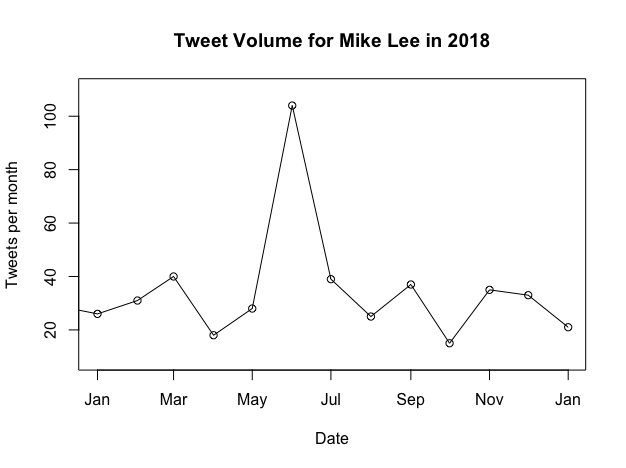
\includegraphics[width =\textwidth]{image/tweet_volume_2018.png}
\caption{Tweet Volume by Month for 2018}
\centering
\end{figure}
\begin{figure}[h!]
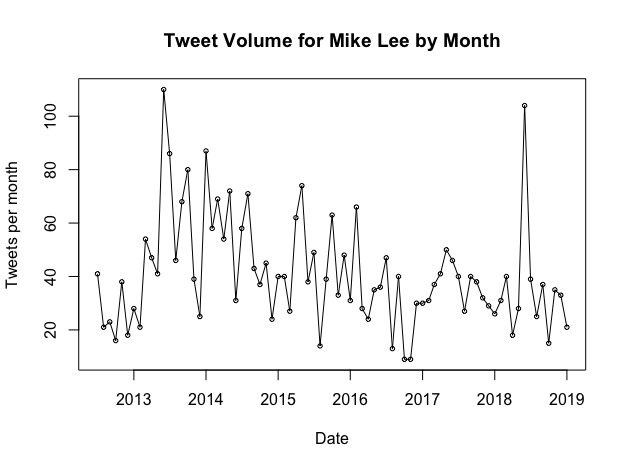
\includegraphics[width =\textwidth]{image/tweet_volume_alltime.png}
\caption{All-Time Tweet Volume by Month}
\centering
\end{figure}
\begin{figure}[h!]
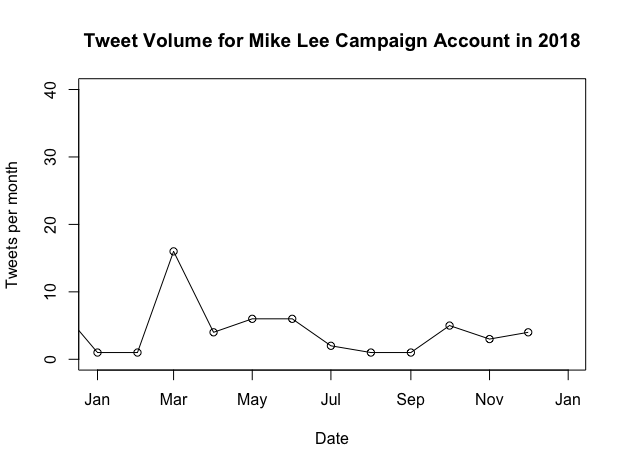
\includegraphics[width =\textwidth]{image/tweet_volume_campaign_2018.png}
\caption{Campaign Tweet Volume by Month for 2018 }
\centering
\end{figure}
\begin{figure}[h!]
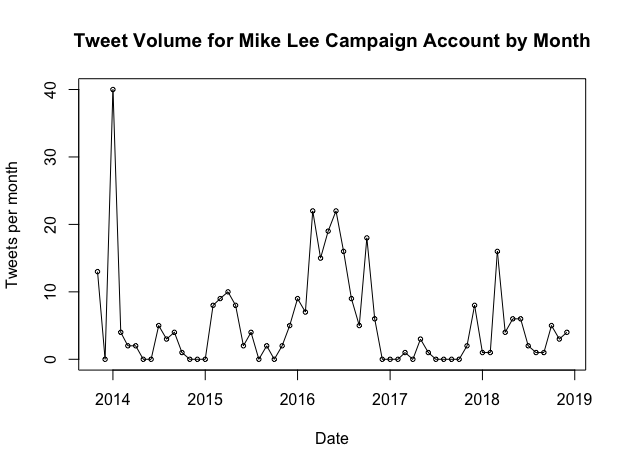
\includegraphics[width =\textwidth]{image/tweet_volume_campaign_alltime.png}
\caption{All-Time Campaign Tweet Volume by Month}
\end{figure}
\begin{figure}[h!]
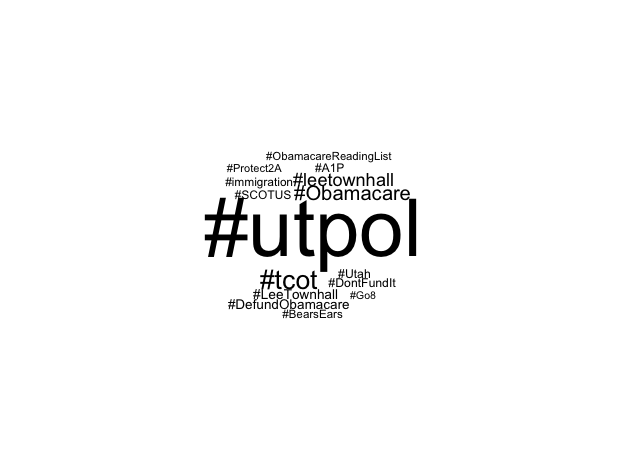
\includegraphics[width =\textwidth]{image/wordpoolht.png}
\caption{Most Common Hashtags Word Cloud}
\end{figure}
\begin{figure}[h!]
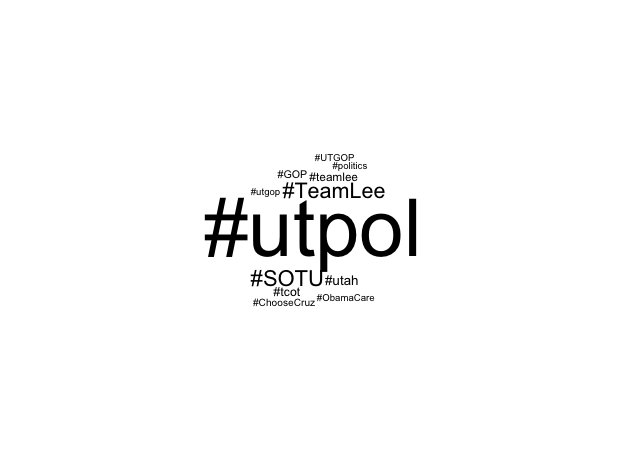
\includegraphics[width =\textwidth]{image/wordcloudht_campaign.png}
\caption{Most Common Campaign Account Hashtags Word Cloud}
\end{figure}
\begin{figure}[h!]
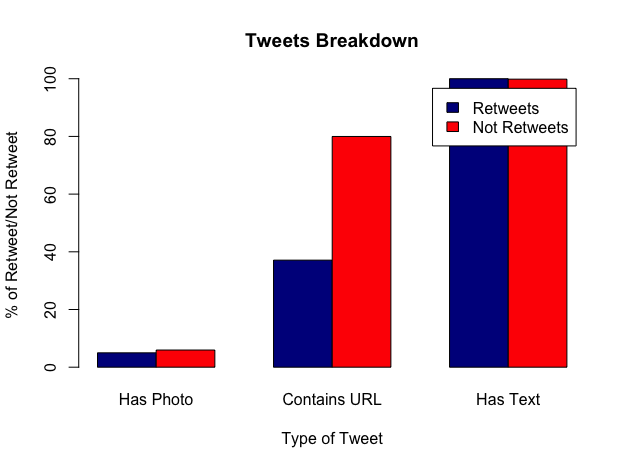
\includegraphics[width =\textwidth]{image/TweetBreakdown.png}
\caption{Tweet Breakdown}
\end{figure}
\begin{figure}[h!]
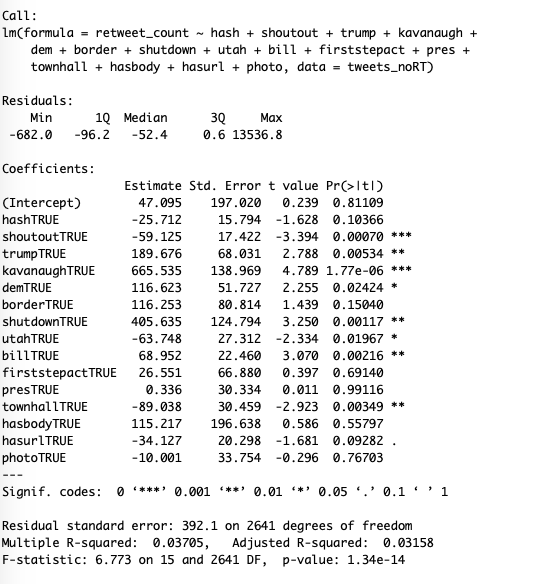
\includegraphics[width =\textwidth]{image/regression_retweet.png}
\caption{Regression Analysis of Re-tweets}
\end{figure}
\begin{figure}[h!]
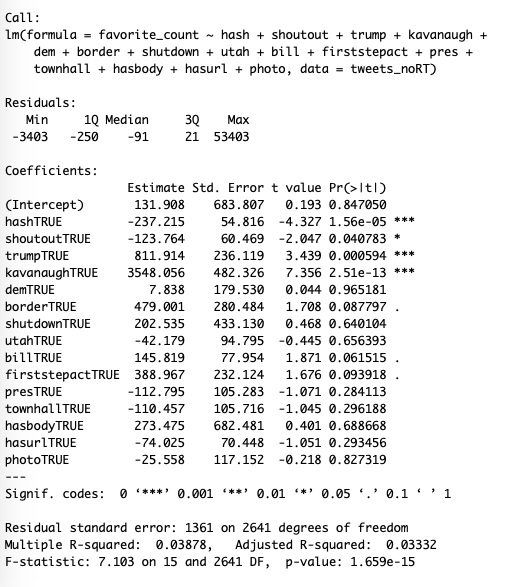
\includegraphics[width =\textwidth]{image/regression_likes.png}
\caption{Regression Analysis of Likes}
\end{figure}
\begin{figure}[h!]
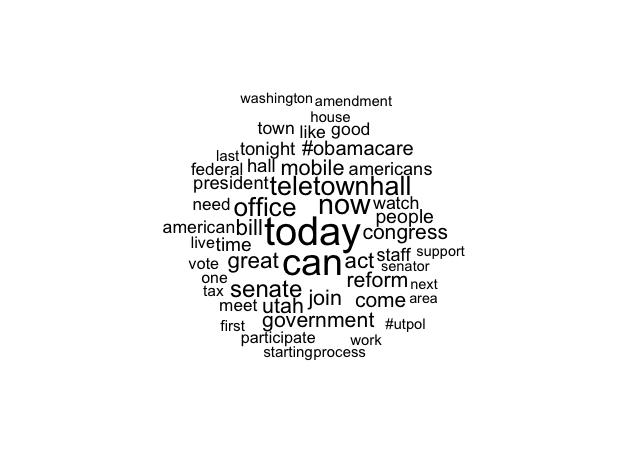
\includegraphics[width =\textwidth]{image/wordcloud.png}
\caption{Word Cloud}
\end{figure}
\begin{figure}[h!]
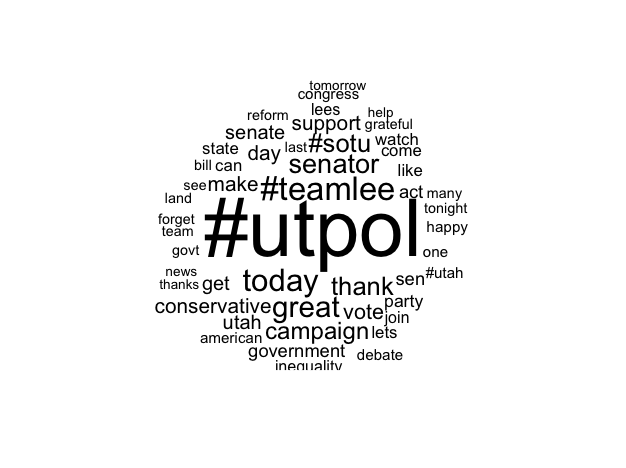
\includegraphics[width =\textwidth]{image/wordcloudcompaign.png}
\caption{Word Cloud of Campaign Account}
\end{figure}
\end{document}
